\begin{itemize}
	\item Нам нужно знать при каких $m$ и $\delta$ наступает равновесие между аннигиляцией и захватом а при каких нет.
\end{itemize}


\begin{figure}[!h]
	\centering
	\only<1>{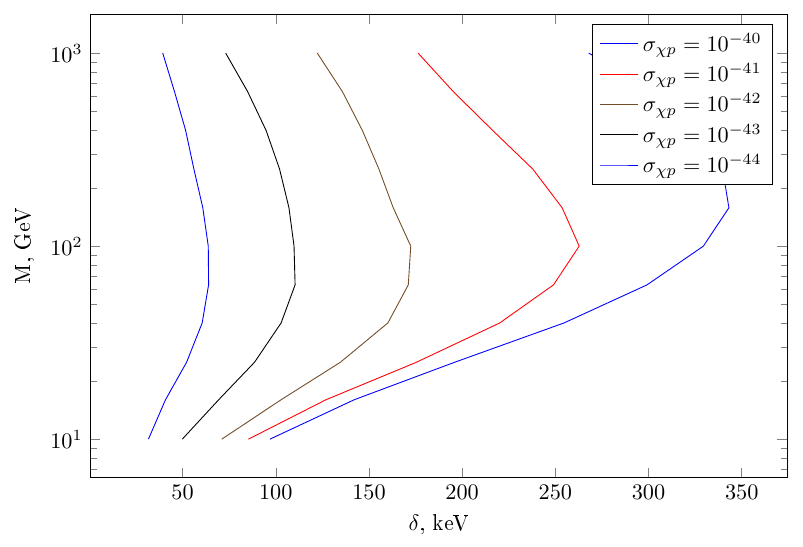
\includegraphics[width=0.65\textwidth]{images/Equilibrium.png}
	\caption{Область параметров $m,\delta$ при которых наступает равновесие между $A$ и $C$ (нераспадающаяся ТМ)}
	}
	\only<2>{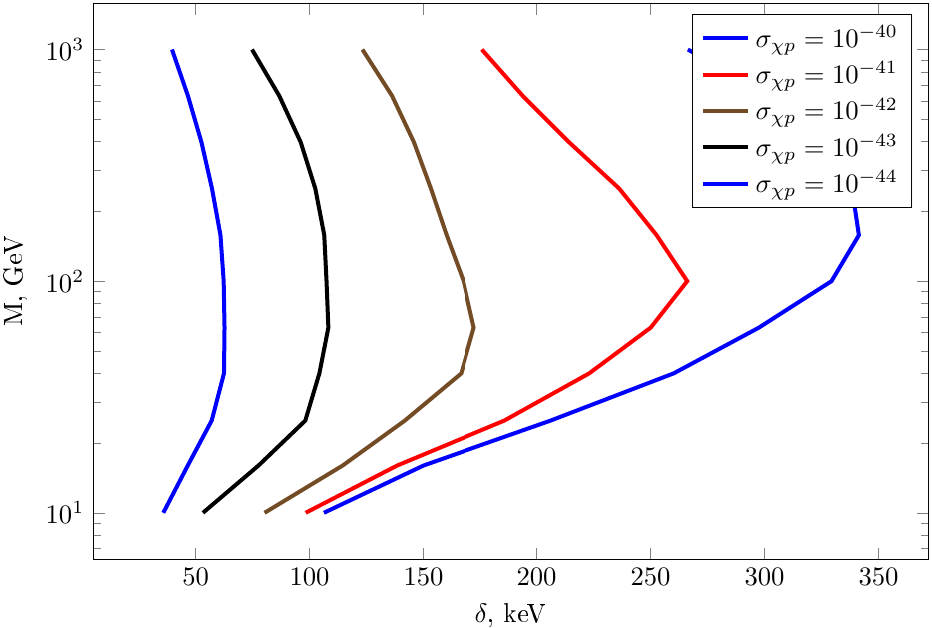
\includegraphics[width=0.65\textwidth]{images/EqFD.png}
	\caption{Область параметров $m,\delta$ при которых наступает равновесие между $A$ и $C$ (распадающаяся ТМ)}
	}
	
\end{figure}
